%  LaTeX support: latex@mdpi.com 
%  In case you need support, please attach all files that are necessary for compiling as well as the log file, and specify the details of your LaTeX setup (which operating system and LaTeX version / tools you are using).

%=================================================================
\documentclass[journal,article,submit,moreauthors,pdftex]{Definitions/mdpi} 

% If you would like to post an early version of this manuscript as a preprint, you may use preprint as the journal and change 'submit' to 'accept'. The document class line would be, e.g., \documentclass[preprints,article,accept,moreauthors,pdftex]{mdpi}. This is especially recommended for submission to arXiv, where line numbers should be removed before posting. For preprints.org, the editorial staff will make this change immediately prior to posting.

%--------------------
% Class Options:
%--------------------
%----------
% journal
%----------
% Choose between the following MDPI journals:
% acoustics, actuators, addictions, admsci, aerospace, agriculture, agriengineering, agronomy, algorithms, animals, antibiotics, antibodies, antioxidants, applsci, arts, asc, asi, atmosphere, atoms, axioms, batteries, bdcc, behavsci , beverages, bioengineering, biology, biomedicines, biomimetics, biomolecules, biosensors, brainsci , buildings, cancers, carbon , catalysts, cells, ceramics, challenges, chemengineering, chemistry, chemosensors, children, cleantechnol, climate, clockssleep, cmd, coatings, colloids, computation, computers, condensedmatter, cosmetics, cryptography, crystals, dairy, data, dentistry, designs , diagnostics, diseases, diversity, drones, econometrics, economies, education, ejihpe, electrochem, electronics, energies, entropy, environments, epigenomes, est, fermentation, fibers, fire, fishes, fluids, foods, forecasting, forests, fractalfract, futureinternet, futurephys, galaxies, games, gastrointestdisord, gels, genealogy, genes, geohazards, geosciences, geriatrics, hazardousmatters, healthcare, heritage, highthroughput, horticulturae, humanities, hydrology, ijerph, ijfs, ijgi, ijms, ijns, ijtpp, informatics, information, infrastructures, inorganics, insects, instruments, inventions, iot, j, jcdd, jcm, jcp, jcs, jdb, jfb, jfmk, jimaging, jintelligence, jlpea, jmmp, jmse, jnt, jof, joitmc, jpm, jrfm, jsan, land, languages, laws, life, literature, logistics, lubricants, machines, magnetochemistry, make, marinedrugs, materials, mathematics, mca, medicina, medicines, medsci, membranes, metabolites, metals, microarrays, micromachines, microorganisms, minerals, modelling, molbank, molecules, mps, mti, nanomaterials, ncrna, neuroglia, nitrogen, notspecified, nutrients, ohbm, optics, particles, pathogens, pharmaceuticals, pharmaceutics, pharmacy, philosophies, photonics, physics, plants, plasma, polymers, polysaccharides, preprints , proceedings, processes, proteomes, psych, publications, quantumrep, quaternary, qubs, reactions, recycling, religions, remotesensing, reports, resources, risks, robotics, safety, sci, scipharm, sensors, separations, sexes, signals, sinusitis, smartcities, sna, societies, socsci, soilsystems, sports, standards, stats, surfaces, surgeries, sustainability, symmetry, systems, technologies, test, toxics, toxins, tropicalmed, universe, urbansci, vaccines, vehicles, vetsci, vibration, viruses, vision, water, wem, wevj

%---------
% article
%---------
% The default type of manuscript is "article", but can be replaced by: 
% abstract, addendum, article, benchmark, book, bookreview, briefreport, casereport, changes, comment, commentary, communication, conceptpaper, conferenceproceedings, correction, conferencereport, expressionofconcern, extendedabstract, meetingreport, creative, datadescriptor, discussion, editorial, essay, erratum, hypothesis, interestingimages, letter, meetingreport, newbookreceived, obituary, opinion, projectreport, reply, retraction, review, perspective, protocol, shortnote, supfile, technicalnote, viewpoint
% supfile = supplementary materials

%----------
% submit
%----------
% The class option "submit" will be changed to "accept" by the Editorial Office when the paper is accepted. This will only make changes to the frontpage (e.g., the logo of the journal will get visible), the headings, and the copyright information. Also, line numbering will be removed. Journal info and pagination for accepted papers will also be assigned by the Editorial Office.

%------------------
% moreauthors
%------------------
% If there is only one author the class option oneauthor should be used. Otherwise use the class option moreauthors.

%---------
% pdftex
%---------
% The option pdftex is for use with pdfLaTeX. If eps figures are used, remove the option pdftex and use LaTeX and dvi2pdf.

%=================================================================
\firstpage{1} 
\makeatletter 
\setcounter{page}{\@firstpage} 
\makeatother
\pubvolume{xx}
\issuenum{1}
\articlenumber{5}
\pubyear{2019}
\copyrightyear{2019}
%\externaleditor{Academic Editor: name}
\history{Received: date; Accepted: date; Published: date}
%\updates{yes} % If there is an update available, un-comment this line

%% MDPI internal command: uncomment if new journal that already uses continuous page numbers 
%\continuouspages{yes}

%------------------------------------------------------------------
% The following line should be uncommented if the LaTeX file is uploaded to arXiv.org
%\pdfoutput=1

%=================================================================
% Add packages and commands here. The following packages are loaded in our class file: fontenc, calc, indentfirst, fancyhdr, graphicx, lastpage, ifthen, lineno, float, amsmath, setspace, enumitem, mathpazo, booktabs, titlesec, etoolbox, amsthm, hyphenat, natbib, hyperref, footmisc, geometry, caption, url, mdframed, tabto, soul, multirow, microtype, tikz

%=================================================================
%% Please use the following mathematics environments: Theorem, Lemma, Corollary, Proposition, Characterization, Property, Problem, Example, ExamplesandDefinitions, Hypothesis, Remark, Definition, Notation, Assumption
%% For proofs, please use the proof environment (the amsthm package is loaded by the MDPI class).

%=================================================================
% Full title of the paper (Capitalized)
\Title{Title}

% Author Orchid ID: enter ID or remove command
\newcommand{\orcidauthorA}{0000-0000-000-000X} % Add \orcidA{} behind the author's name
%\newcommand{\orcidauthorB}{0000-0000-000-000X} % Add \orcidB{} behind the author's name

% Authors, for the paper (add full first names)
\Author{Valentina Aleotti $^{1}$*, Amin Ravaei $^{1}$, Vincenza Colonna $^{3}$,  Orsola Brasile $^{2}$, Roberta Capucci $^{2}$ and Michele Rubini $^{1}$\orcidA{}}

% Authors, for metadata in PDF
\AuthorNames{Firstname Lastname, Firstname Lastname and Firstname Lastname}

% Affiliations / Addresses (Add [1] after \address if there is only one affiliation.)
\address{%
$^{1}$ \quad Department of Biomedical and Specialty Surgical Sciences, Section of Medical Biochemistry, Molecular Biology and Genetics, University of Ferrara, Ferrara, Italy. \\
$^{2}$ \quad Department of Morphology, Surgery and Experimental Medicine, Section of Obstetrics and Gynecology, Ferrara, Italy.\\
$^{3}$ \quad Institute of Genetics and Biophysics, Consiglio Nazionale di Ricerche, Naples, Italy.}

% Contact information of the corresponding author
\corres{Correspondence: lttvnt@unife.it}

% Current address and/or shared authorship
%\firstnote{Current address: Affiliation 3} 
%\secondnote{These authors contributed equally to this work.}
% The commands \thirdnote{} till \eighthnote{} are available for further notes

%\simplesumm{} % Simple summary

%\conference{} % An extended version of a conference paper

% Abstract (Do not insert blank lines, i.e. \\) 
\abstract{Recurrent pregnancy loss (RPL) is specified as two or more consecutive spontaneous loss of pregnancy. In 50\% of the cases, the causes of RPL are still unknown. The aims of this study is to understand if the genetic and epigenetic profile in the women and, for the first time, on the product of conception play a role in determining the risk of RPL. This study analyses 156 Volunteer termination pregnancy (VTP) and 131 cases of RPL. The results shows that SNP rs1801133 in MTHFR gene is associated in recessive homozygote women with significant increased risk of RPL under a co-dominant model (p=0.004). In embryos the recessive genotype at the SNP rs2617170 in NKG2D gene shows a protective effect from RPL (p=0.0067). The anaylsis of methylation of DNA show a significant increase of methylation level (p=0.0010) in RPL cases compared to VTP cases in chorionic villi. When considering the exposure to periconceptional supplementation with folic acid (FA), the LINE-1 DNA methylation among RPL cases in CV is significantly higher in cases not supplemented with FA (p= 0.030). This study shows the importance to identify an effective protocol for the treatment of women with RPL without apparent cause that currently is absent.}

%A single paragraph of about 200 words maximum. For research articles, abstracts should give a pertinent overview of the work. We strongly encourage authors to use the following style of structured abstracts, but without headings: (1) Background: Place the question addressed in a broad context and highlight the purpose of the study; (2) Methods: Describe briefly the main methods or treatments applied; (3) Results: Summarize the article's main findings; and (4) Conclusion: Indicate the main conclusions or interpretations. The abstract should be an objective representation of the article, it must not contain results which are not presented and substantiated in the main text and should not exaggerate the main conclusions.

% Keywords
\keyword{Miscarriage; Product of conception; Epigenetic; Recurrent pregnancy loss; Genetic; LINE-1 methylation;Folic acid supplementation}

% The fields PACS, MSC, and JEL may be left empty or commented out if not applicable
%\PACS{J0101}
%\MSC{}
%\JEL{}

%%%%%%%%%%%%%%%%%%%%%%%%%%%%%%%%%%%%%%%%%%
% Only for the journal Diversity
%\LSID{\url{http://}}

%%%%%%%%%%%%%%%%%%%%%%%%%%%%%%%%%%%%%%%%%%
% Only for the journal Applied Sciences:
%\featuredapplication{Authors are encouraged to provide a concise description of the specific application or a potential application of the work. This section is not mandatory.}
%%%%%%%%%%%%%%%%%%%%%%%%%%%%%%%%%%%%%%%%%%

%%%%%%%%%%%%%%%%%%%%%%%%%%%%%%%%%%%%%%%%%%
% Only for the journal Data:
%\dataset{DOI number or link to the deposited data set in cases where the data set is published or set to be published separately. If the data set is submitted and will be published as a supplement to this paper in the journal Data, this field will be filled by the editors of the journal. In this case, please make sure to submit the data set as a supplement when entering your manuscript into our manuscript editorial system.}

%\datasetlicense{license under which the data set is made available (CC0, CC-BY, CC-BY-SA, CC-BY-NC, etc.)}

%%%%%%%%%%%%%%%%%%%%%%%%%%%%%%%%%%%%%%%%%%
% Only for the journal Toxins
%\keycontribution{The breakthroughs or highlights of the manuscript. Authors can write one or two sentences to describe the most important part of the paper.}

%\setcounter{secnumdepth}{4}
%%%%%%%%%%%%%%%%%%%%%%%%%%%%%%%%%%%%%%%%%%
\begin{document}
%%%%%%%%%%%%%%%%%%%%%%%%%%%%%%%%%%%%%%%%%%

%%%%%%%%%%%%%%%%%%%%%%%%%%%%%%%%%%%%%%%%%%
%\setcounter{section}{-1} %% Remove this when starting to work on the template.
%\section{How to Use this Template}
%The template details the sections that can be used in a manuscript. Note that the order and names of article sections may differ from the requirements of the journal (e.g., the positioning of the Materials and Methods section). Please check the instructions for authors page of the journal to verify the correct order and names. For any questions, please contact the editorial office of the journal or support@mdpi.com. For LaTeX related questions please contact latex@mdpi.com.
%The order of the section titles is: Introduction, Materials and Methods, Results, Discussion, Conclusions for these journals: aerospace,algorithms,antibodies,antioxidants,atmosphere,axioms,biomedicines,carbon,crystals,designs,diagnostics,environments,fermentation,fluids,forests,fractalfract,informatics,information,inventions,jfmk,jrfm,lubricants,neonatalscreening,neuroglia,particles,pharmaceutics,polymers,processes,technologies,viruses,vision

\section{Introduction}
%The introduction should briefly place the study in a broad context and highlight why it is important. It should define the purpose of the work and its significance. The current state of the research field should be reviewed carefully and key publications cited. Please highlight controversial and diverging hypotheses when necessary. Finally, briefly mention the main aim of the work and highlight the principal conclusions. As far as possible, please keep the introduction comprehensible to scientists outside your particular field of research. Citing a journal paper \cite{ref-journal}. And now citing a book reference \cite{ref-book}. Please use the command \citep{ref-journal} for the following MDPI journals, which use author-date citation: Administrative Sciences, Arts, Econometrics, Economies, Genealogy, Humanities, IJFS, JRFM, Languages, Laws, Religions, Risks, Social Sciences.

\noindent Pregnancy loss (PL) is defined by \textit{World Health Organization} (\textbf{WHO}) as the loss of pregnancy resulting in fetal death before 20-28 weeks and by Italian law as the natural interruption of pregnancy caused by pathologies. In particular, any expulsion or fetal/embryo death occurring within 180 days (25 weeks and 5 days) (\textbf{ISTAT}). Roughly 10-15 \% of all clinically recognized pregnancies result in miscarriage. Recurrent pregnancy loss (RPL) denotes two or more consecutive spontaneous loss of pregnancy happening within 20-24 weeks of gestation. RPL affects at least 1-2\% of women in reproductive age. Most of the miscarriages happens during the first trimester of gestation. The main known causes of RPL are chromosomal anomalies, anatomical abnormalities, autoimmune diseases, infection diseases, advanced maternal and paternal age and environmental agents. In 50\% of cases, the causes of RPL are still unknown \cite{campana2017association, du2019polymorphisms, sudhir2016cytogenetic, oliver2014diagnosis, yakut2015chromosome}. The diagnosis of miscarriages is based on embryo heart activity and gestational sac features revealed by ultrasonography. However, the diagnosis takes place only after the death of the embryo, and only a few cases are followed to understand the genetic causes with appropriate techniques. The protocols to treat this pathology provide a committed and focused service to couples who already had experience of RPL, so it doesn’t prevent from a new event of miscarriage. In literature are reported a lot of SNPs that are linked to increase the risk of miscarriage. One of this, is \textit{NKG2D} (c.311A\textgreater{}G) rs2617170. This gene is a member of group of genes where their expression is mostly in natural kill (NK) cells. These types of cell have an important function in the maintenance of pregnancy. In mothers with recessive genotype for this SNP confers a high cytotoxic activity that can induce RPL. Another gene involved in RPL is \textit{MTHFR} c.677C \textgreater{}T rs1801133 in strictly correlation with pathway of production of folic acid. The  enzyme MTHFR plays  a decisive  role  in  the  folate  metabolism  pathway  and regulates the intracellular folate pool for synthesis and methylation of DNA. Due to its role in methylation, we wanted to study the epigenetic. DNA methylation is the most studied type of epigenetic mark. In particular, the sequence of LINE-1 and its methylation due to their high genome dissemination (20\%), is a surrogate marker of global DNA methylation level. Scientific evidence increasingly suggests that exposures during the intrauterine period can increase the danger of developing disease in later life. One of this exposition is folic acid in early pregnancy may have important and lasting effects on DNA methylation  and  consequently  influence  gene  expression  and  disease phenotype across the life course. The aims of this study is to understand if the genetic and epigenetic profile in the women and, for the first time, on the product of conception play a role in determining the risk of Recurrent Pregnancy Loss (RPL). \\
 
%%%%%%%%%%%%%%%%%%%%%%%%%%%%%%%%%%%%%%%%%%
\section{Results}

%This section may be divided by subheadings. It should provide a concise and precise description of the experimental results, their interpretation as well as the experimental conclusions that can be drawn.
%\begin{quote}
%This section may be divided by subheadings. It should provide a concise and precise description of the experimental results, their interpretation as well as the experimental conclusions that can be drawn.
%\end{quote}


%%%%%%%%%%%%%%%%%%%%%%%%%%%%%%%%%%%%%%%%%%

%\subsection{Genetic association between polymorphism in the genes under study and RPL }
\subsection{Genetic association between polymorphism in the genes under study and RPL }

%\noindent In this genetic association case-control study, we compared the frequency of allele and genotypes at specific genetic marker loci (SNPs), in individuals from mothers and chorionic villi (CV) with recurrent pregnancy loss (RPL) and mothers and CV with volunteer termination pregnancy (VTP) in order to determine whether a statistical association exists beetween the RPL and the SNPs. 
\noindent To determine if there is association between alleles at single nucleotide polymorphic sites (SNPs) in eight genes previously associated with RPL, we performed a case-control study between mothers and embryos for RPL and voluntary termination of pregnancy 

, comparing the frequencies of allele and genotypes at specific genetic marker loci (SNPs), in individuals from mothers and chorionic villi (CV) with recurrent pregnancy loss (RPL) and mothers and CV with volunteer termination pregnancy (VTP) in order to determine whether a statistical association exists beetween the RPL and the SNPs. 
In table \ref{tab:pannel of genes}, we describe the SNPs linked to the risk of miscarriage, selected after extensively searching in the literature. In brief, these genes are correlated with embryo's develope. The analyses done in this chapter follows guideline for statistical analysis for case-control study of \textit{ Clarke GM. et al.,2011} \cite{clarke2011basic}. In 15\% of samples, genotyping was repeated for quality testing. The indeterminate samples and the maternal and fetous genotypes discordant were excluded by the analysis.The first step of the association analysis was to evaluate if the SNPs were in HWE and when considering a threshold for significance of 0.05 in global evaluation all the loci are in HWE, since their observed genotypic frequencies are not significantly different from the expected one, therefore all the SNP were used for subsequent analyses. All the SNPs used for this studied have a MAF> 5-10\%.

\unskip
\subsubsection{Odds ratio of the alleles and genotype under co-dominant model}


\noindent All the SNP considered have two alleles, of which the most frequent in the general population according to Ensembl Release 99 (January 2020)[www.ensembl.org] was considered dominant. We calculated the ratio of the odds of disease in RPL carrying the recessive allele compared with RPL carrying the dominant one under a model of co-dominance. The results are shown in table \ref{tab:Allele analysis in WBC and CV} for both WBC and CV. In WBC, the results indicates that c.677T allele of the gene \textit{MTHFR} rs1801133 associates in mothers with significant increased risk of RPL (OR= 1.72, p=0.0018) following a co-dominant model. In the rest of SNP in WBC no other p-value is significant. For CV, there is significant result for the gene \textit{NKG2D} rs2617170, where the recessive allele seems to protect embryo from RPL (OR=0.64, p=0.025). No other SNP is significant. We calculated the ratio of the odds of disease in RPL carrying homozygous and heterozygous genotypes for the recessive allele compared with RPL carrying the homozygous dominant genotype under a model of co-dominance. The results for both WBC and CV are shown in table \ref{tab:Model genetic analysis in WBC and CV}. Of all the SNP considered, two show significant association with risk or protection in mothers (WBC) and embryos (CV), while the other SNPs instead seems to have no association with RPL. Details of the ORs for the rs1801133 SNP in the \textit{MTHFR} gene WBC, indicates that c.677T allele in mothers associates with significant increased risk of RPL (OR= 1.72, p=0.0018) following a co-dominant model, with an almost 3-fold increased risk in T/T homozygote women (OR=2.64, p=0.004), and a lower risk in heterozygotes (OR=1.61, p=0.075). Similarly, the recessive genotype in gene \textit{NKG2D}, seems protect embryo from RPL (OR=0.27, p=0.0067 ).

\subsection{Analysis of methylation pattern of the LINE-1 sequence}

\noindent For the analysis on the level of methylation in LINE-1 sequence, we used a normality test called \textit{"Shapiro Wilk test"} for check if the dates followed a normal distribution. The Shapiro-Wilk test showed that WBC samples in RPL (W=0.98, p-value= 0.64) and VTP (W=0.97, p-value= 0.080) followed a normal distribution of LINE-1 methylation. Instead, for CV samples, the RPL (W=0.89, p=3.96*10-5) and VTP (W=0.93, p=0.0006) not followed a normal distribution, as describe in table \ref{tab:Normality test}. The samples are aged matched for exclude a bias in the analyses: the age limit for embryo in RPL and VTP is 90 days. \\

\noindent Afterwards, we calculated the mean of RPL in WBC and the 77\% (sd=0.41\%) of CpG island is metilated. For CV of RPL, the mean is 60\% (sd=1.0\%). As control, in VTP we see that the 78\% (sd=0.62\%) of CpG island is metilated and in CV, the mean is 55\% (sd=0.83\%), as describe in table \ref{tab:methylation level}. The difference from two group in WBC is not significant (T student test p-value= 0.70). In CV, appears significant the fact that in the RPL, it seems more ipermethylated than control (Mann-Whitney p-value= 0.0010). %The Figure \ref{fig:Global methylation} shows a box plot of the difference on methylation. On the left, there is the global methylation in WBC, in red for RPL and in blue for VTP. On the right, are represented the CV, with is visible more difference in mean of methylation.\\
\noindent After this evaluation, for the following analysis of stratification, an unpaired student t test was used for WBC that followed a normal distribution. For CV sample that not followed a normal distribution, we used a non parametric test called "\textit{Mann-Whitney test}". The analyses done in this chapter follows the statistical analysis for LINE-1 methylation study of \textit{Khan MFJ. et al.,2017} \cite{khan2018evaluating}. \\

\noindent Analyzing the stratification of the DNA methylation on different parameter present in clinical database, there is a comparison between RPL and VTP samples of CV and WBC on the average of LINE-1 methylation level. The parameters analyzed were the age of mothers, BMI of mothers, smoking exposure, folic acid intake and embryo age and sex (table \ref{tab:LINE-1 methylation on clinical data}). For comparison of this parameters, the unpaired student’s t-test for WBC and Mann-Whitney test for CV were performed.  

\noindent The folic acid (FA) intake is considered if women used folic acid during pregnancy or not. As shows in table \ref{tab:LINE-1 methylation on clinical data}, the mean of RPL in WBC with FA is 77\% (sd=0.45\%) against the RPL without intake of FA where mean is 77\% (sd=0.38\%), there is no difference (t-student p-value= 0.97). \\

\noindent In CV, the mean of RPL with FA is 57\% (sd=0.81\%) against the RPL without intake of FA where mean is 62\% (sd=1.0\%), there is a significant difference (Mann-Whitney p-value= 0.030), as shows in figure \ref{fig:FA CV}. In VTP, no women intakes folic acid, because the pregnancy probably was not planned, so we can't apply the Mann-Whitney test because we don't have any case of VTP with folic acid supplementation.


%\unskip
%\subsubsection{Subsubsection}

%Bulleted lists look like this:
%\begin{itemize}[leftmargin=*,labelsep=5.8mm]
%\item	First bullet
%\item	Second bullet
%\item	Third bullet
%\end{itemize}

%Numbered lists can be added as follows:
%\begin{enumerate}[leftmargin=*,labelsep=4.9mm]
%\item	First item 
%\item	Second item
%\item	Third item
%\end{enumerate}

\subsection{Figures, Tables and Schemes}

%All figures and tables should be cited in the main text as Figure 1, Table 1, etc.

%\begin{figure}[H]
%\centering
%
\includegraphics[width=2 cm]{Definitions/logo-mdpi}
%\caption{This is a figure, Schemes follow the same formatting. If there are multiple panels, they should be listed as: (\textbf{a}) Description of what is contained in the first panel. (\textbf{b}) Description of what is contained in the second panel. Figures should be placed in the main text near to the first time they are cited. A caption on a single line should be centered.}
%\end{figure}  


\begin{table}[H]
\caption{Pannel of candidate variants genes analyzed with major and minor allele, ancestral allele, derived allele and the chromosomes position}
\centering
 \resizebox{\textwidth}{!}{
\begin{tabular}{ccccccl}
\hline
\textit{\textbf{Gene}} &
  \textit{\textbf{rsID}} &
  \textit{\textbf{Major/minor allele}} &
  \textit{\textbf{\begin{tabular}[c]{@{}c@{}}Ancestral\\ allele\end{tabular}}} &
  \textit{\textbf{Derived allele}} &
  \textit{\textbf{\begin{tabular}[c]{@{}c@{}}Chromosome \\ position\end{tabular}}} &
  \multicolumn{1}{c}{\textit{\textbf{Role}}} \\ \hline
MTHFR &
  rs1801133 &
  C/T &
  C &
  C|C, C|T, T|T &
  1:11796321 &
  Metabolism folic acid \cite{liew2015methylenetetrahydrofolate} \\ \hline
MTHFR &
  rs1801131 &
  A/C &
  A &
  A|A, A|C, C|C &
  1:11794419 &
  Metabolism folic acid\cite{kim2006influence} \\ \hline
HLA-G  &
 rs371194629 &
  14bp Del/Ins &
  NA &
  D|D, D|I, I|I &
  6:29830804 &
  Immune tolerance in pregnancy \cite{nowak2016possible}\cite{arjmand2016balance}\cite{alassociation} \\ \hline
ANXA5 &
  rs1050606 &
  A/C &
  C &
  A|A, A|C, C|C &
  4:121696891 &
  Ca2+ dependent placenta anticoagulant protein \cite{hayashi2013genotyping} \cite{zhang2017association} \\ \hline
NKG2D &
  rs2617170 &
  A/G &
  A &
  G|G, G|A, A|A &
  12:10408358 &
  Detection and elimination of transformed and infected cells \cite{hizem2014polymorphisms} \\ \hline
IL-10 &
  rs1800871 &
  A/G &
  G &
  G|G, G|A, A|A &
  1:206773289 &
  Cytokines in the cascade of immune signalling \cite{cochery2009interleukin} \cite{qaddourah201410} \\ \hline
CTLA-4 &
  rs231775 &
  A/G &
  A &
  G|G, G|A, A|A &
  2:203867991 &
  Member of immunoglobulin superfamily \cite{misra2016association} \\ \hline
SMTH1 &
  rs1979277 &
  C/T &
  C &
  C|C, C|T, T|T &
  17:18328782 &
  Metabolism folic acid \cite{engel2006polymorphisms} \\ \hline
PLK4 &
  rs2305957 &
  A/G &
  G &
  G|G, G|A, A|A &
  4:127811771 &
  Regulates centriole duplication during cell cycle \cite{zhang2017maternal}\cite{mccoy2015common} \\ \hline
\end{tabular}
}
\label{tab:pannel of genes}
\end{table}


\begin{table}[H]
\caption{Odds ratio of disease in RPL carrying the R recessive allele compared with RPL carrying the dominant one \textbf{D}, under a model of co-dominance in WBC and CV}
\centering
\resizebox{\textwidth}{!}{%
\begin{tabular}{clllccccl}
\hline
\multicolumn{5}{c}{\textbf{Allele analysis in WBC}} &
  \multicolumn{4}{c}{\textbf{Allele analysis in CV}} \\ \hline
\textit{\textbf{SNP}} &
  \multicolumn{1}{c}{\textit{\textbf{RPL}}} &
  \multicolumn{1}{c}{\textit{\textbf{VTP}}} &
  \multicolumn{1}{c}{\textit{\textbf{OR (IC 95\%)}}} &
  \textit{\textbf{p-value}} &
  \textit{\textbf{RPL}} &
  \textit{\textbf{VTP}} &
  \textit{\textbf{OR (IC 95\%)}} &
  \multicolumn{1}{c}{\textit{\textbf{p-value}}} \\ \hline
\textit{\textbf{MTHFR rs1801133}} &
   &
   &
   &
  \multicolumn{1}{l}{} &
  \multicolumn{1}{l}{} &
  \multicolumn{1}{l}{} &
  \multicolumn{1}{l}{} &
   \\ \hline
\textit{\textbf{D}} &
  138 &
  207 &
  1.00 (Reference) &
  \multicolumn{1}{l}{} &
  121 &
  186 &
  1.00 (Reference) &
   \\ \hline
\textit{\textbf{R}} &
  114 &
  99 &
  1.72(1.22-2.43) &
  \multicolumn{1}{l}{\textbf{0.0018}} &
  81 &
  104 &
  1.19(0.82-1.73) &
  \multicolumn{1}{c}{0.33} \\ \hline
\textit{\textbf{MTHFR rs1801131}} &
  \multicolumn{1}{c}{} &
  \multicolumn{1}{c}{} &
  \multicolumn{1}{c}{} &
   &
  \multicolumn{1}{l}{} &
  \multicolumn{1}{l}{} &
  \multicolumn{1}{l}{} &
   \\ \hline
\textit{\textbf{D}} &
  \multicolumn{1}{c}{173} &
  \multicolumn{1}{c}{201} &
  \multicolumn{1}{c}{1.00 (Reference)} &
   &
  138 &
  205 &
  1.00 (Reference) &
   \\ \hline
\textit{\textbf{R}} &
  \multicolumn{1}{c}{77} &
  \multicolumn{1}{c}{103} &
  \multicolumn{1}{c}{0.86(0.60-1.24)} &
  0.44 &
  62 &
  85 &
  1.083(0.73-1.60) &
  \multicolumn{1}{c}{0.68} \\ \hline
\textit{\textbf{HLA-G 14bp}} &
   &
   &
   &
   &
  \multicolumn{1}{l}{} &
  \multicolumn{1}{l}{} &
  \multicolumn{1}{l}{} &
   \\ \hline
\textit{\textbf{D}} &
  132 &
  161 &
  1.00 (Reference) &
   &
  121 &
  157 &
  1.00 (Reference) &
  \multicolumn{1}{c}{} \\ \hline
\textit{\textbf{R}} &
  120 &
  137 &
  1.068(0.76-1.49) &
  0.69 &
  81 &
  125 &
  0.84(0.58-1.21) &
  \multicolumn{1}{c}{0.35} \\ \hline
\textit{\textbf{ANXA5 rs1050606}} &
   &
   &
   &
   &
  \multicolumn{1}{l}{} &
  \multicolumn{1}{l}{} &
  \multicolumn{1}{l}{} &
   \\ \hline
\textit{\textbf{D}} &
  124 &
  148 &
  1.00(Reference) &
   &
  107 &
  147 &
  \multicolumn{1}{l}{1.00 (Reference)} &
   \\ \hline
\textit{\textbf{R}} &
  126 &
  150 &
  1.002(0.71-1.39) &
  0.98 &
  95 &
  143 &
  0.91(0.63-1.30) &
  \multicolumn{1}{c}{0.61} \\ \hline
\textit{\textbf{NKG2D rs2617170}} &
   &
   &
   &
   &
  \multicolumn{1}{l}{} &
  \multicolumn{1}{l}{} &
  \multicolumn{1}{l}{} &
   \\ \hline
\textit{\textbf{D}} &
  165 &
  192 &
  1.00(Reference) &
   &
  141 &
  174 &
  \multicolumn{1}{l}{1.00 (Reference)} &
   \\ \hline
\textit{\textbf{R}} &
  83 &
  112 &
  0.86(0.60-1.22) &
  0.40 &
  61 &
  116 &
  0.64(0.44-0.95) &
  \multicolumn{1}{c}{\textbf{0.025}} \\ \hline
\textit{\textbf{IL-10 rs1800871}} &
   &
   &
   &
   &
  \multicolumn{1}{l}{} &
  \multicolumn{1}{l}{} &
  \multicolumn{1}{l}{} &
   \\ \hline
\textit{\textbf{D}} &
  191 &
  210 &
  1.00(Reference) &
   &
  143 &
  194 &
  1.00 (Reference) &
   \\ \hline
\textit{\textbf{R}} &
  59 &
  88 &
  0.73(0.50-1.081) &
  0.11 &
  57 &
  88 &
  0.87(0.59-1.30) &
  \multicolumn{1}{c}{0.52} \\ \hline
\textit{\textbf{CTLA-4 rs231775}} &
   &
   &
   &
  \multicolumn{1}{l}{} &
  \multicolumn{1}{l}{} &
  \multicolumn{1}{l}{} &
  \multicolumn{1}{l}{} &
   \\ \hline
\textit{\textbf{D}} &
  167 &
  211 &
  1.00(Reference) &
   &
  139 &
  192 &
  \multicolumn{1}{l}{1.00 (Reference)} &
   \\ \hline
\textit{\textbf{R}} &
  81 &
  93 &
  1.10(0.76-1.57) &
  0.60 &
  61 &
  96 &
  0.87(0.60-1.40) &
  \multicolumn{1}{c}{0.50} \\ \hline
\textit{\textbf{SMTH1 rs1979277}} &
   &
   &
   &
   &
   &
   &
  \multicolumn{1}{l}{} &
   \\ \hline
\textit{\textbf{D}} &
  194 &
  223 &
  1.00(Reference) &
   &
  155 &
  211 &
  1.00 (Reference) &
   \\ \hline
\textit{\textbf{R}} &
  56 &
  71 &
  0.90(0.60-1.35) &
  0.63 &
  43 &
  75 &
  0.78(0.50-1.19) &
  \multicolumn{1}{c}{0.25} \\ \hline
\textit{\textbf{PLK4 rs2305957}} &
   &
   &
   &
   &
   &
   &
  \multicolumn{1}{l}{} &
   \\ \hline
\textit{\textbf{D}} &
  187 &
  226 &
  1.00(Reference) &
   &
  153 &
  217 &
  1.00 (Reference) &
   \\ \hline
\textit{\textbf{R}} &
  61 &
  64 &
  1.15(0.77-1.71) &
  0.48 &
  47 &
  73 &
  \multicolumn{1}{l}{0.91(0.44-0.95)} &
  \multicolumn{1}{c}{0.67} \\ \hline
\end{tabular}%
}
\label{tab:Allele analysis in WBC and CV}
\end{table}



\begin{table}[H]
\caption{Odds ratio and confidence intervals with p-value calculated under a model of co-dominance for the heterozygous DR and homozygous recessive RR genotypes at the considered genetic loci. Data relative to \textit{MTHFR} rs1801133 in WBC on the left and to \textit{NKG2D} rs2617170 in CV on the right.}
\centering
\resizebox{\textwidth}{!}{%
\begin{tabular}{ccccccccc}
\hline
\multicolumn{5}{c}{\textbf{Co-dominant model in WBC}} &
  \multicolumn{4}{c}{\textbf{Co-dominant model in CV}} \\ \hline
\textit{\textbf{SNP}} &
  \textit{\textbf{RPL}} &
  \textit{\textbf{VTP}} &
  \textit{\textbf{OR (IC 95\%)}} &
  \textit{\textbf{p-value}} &
  \textit{\textbf{RPL}} &
  \textit{\textbf{VTP}} &
  \textit{\textbf{OR (IC 95\%)}} &
  \textit{\textbf{p-value}} \\ \hline
\textit{\textbf{MTHFR rs1801133}}  &    &    &                   &       &    &    &                  &      \\ \hline
\textit{\textbf{DD}}         & 42 & 74 & 1.00 (Reference)  &       & 34 & 60 & 1.00 (Reference) &      \\ \hline
\textit{\textbf{DR}}         & 54 & 59 & 1.61(0.95-2.73)   & 0.075 & 53 & 66 & 1.41(0.81-2.46   & 0.21 \\ \hline
\textit{\textbf{RR}}         & 30 & 20 & 2.64(1.33-5.22)   & \textbf{0.004} & 14 & 19 & 1.30(0.57-2.91)  & 0.52 \\ \hline
\textit{\textbf{MTHFR rs1801131}}  &    &    &                   &       &    &    &                  &      \\ \hline
\textit{\textbf{DD}}         & 65 & 69 & 1.00 (Reference)  &       & 48 & 71 & 1.00 (Reference) &      \\ \hline
\textit{\textbf{DR}}         & 43 & 63 & 0.72(0.43-1.21)   & 0.21  & 42 & 63 & 0.98(0.57-1.68)  & 0.95 \\ \hline
\textit{\textbf{RR}}         & 17 & 20 & 0.90(0.43-1.87)   & 0.78  & 10 & 11 & 1.34(0.52-3.41)  & 0.53 \\ \hline
\textit{\textbf{HLA-G 14bp}} &    &    &                   &       &    &    &                  &      \\ \hline
\textit{\textbf{DD}}         & 33 & 43 & 1.00 (Reference)  &       & 39 & 46 & 1.00 (Reference) &      \\ \hline
\textit{\textbf{DR}}         & 66 & 75 & 1.14(0.65-2.01)   & 0.63  & 43 & 65 & 0.78(0.43-1.38)  & 0.39 \\ \hline
\textit{\textbf{RR}}         & 27 & 31 & 1.13(0.57-2.25)   & 0.71  & 19 & 30 & 0.74 (0.36-1.52) & 0.42 \\ \hline
\textit{\textbf{ANXA5 rs1050606}}  &    &    &                   &       &    &    &                  &      \\ \hline
\textit{\textbf{DD}}         & 31 & 39 & 1.00(Reference)   &       & 35 & 44 & 1.00 (Reference) &      \\ \hline
\textit{\textbf{DR}}         & 62 & 70 & 1.14(0.65-2.010)  & 0.71  & 37 & 59 & 0.78(0.43-1.38)  & 0.44 \\ \hline
\textit{\textbf{RR}}         & 32 & 40 & 1.0064(0.51-1.95) & 0.98  & 29 & 42 & 0.86(0.45-1.66)  & 0.66 \\ \hline
\textit{\textbf{NKG2D rs2617170}}  &    &    &                   &       &    &    &                  &      \\ \hline
\textit{\textbf{DD}}         & 54 & 61 & 1.00(Reference)   &       & 46 & 55 & 1.00 (Reference) &      \\ \hline
\textit{\textbf{DR}}         & 57 & 70 & 0.91(0.55-1.52)   & 0.74  & 49 & 64 & 0.91(0.53-1.57)  & 0.74 \\ \hline
\textit{\textbf{RR}} &
  13 &
  21 &
  0.69(0.31-1.52) &
  0.36 &
  6 &
  26 &
  0.27(0.10-0.72) &
  \textbf{0.0067} \\ \hline
\textit{\textbf{IL-10 rs1800871}}  &    &    &                   &       &    &    &                  &      \\ \hline
\textit{\textbf{DD}}         & 70 & 71 & 1.00(Reference)   &       & 54 & 65 & 1.00 (Reference) &      \\ \hline
\textit{\textbf{DR}}         & 51 & 68 & 0.76(0.46-1.24)   & 0.27  & 35 & 64 & 0.65(0.38-1.13)  & 0.13 \\ \hline
\textit{\textbf{RR}}         & 4  & 10 & 0.40(0.61-1.35)   & 0.13  & 11 & 12 & 1.10(0.45-2.69)  & 0.82 \\ \hline
\textit{\textbf{CTLA-4 rs231775}}   &    &    &                   &       &    &    &                  &      \\ \hline
\textit{\textbf{DD}}         & 55 & 70 & 1.00(Reference)   &       & 45 & 58 & 1.00 (Reference) &      \\ \hline
\textit{\textbf{DR}}         & 57 & 71 & 1.021(0.62-1.67)  & 0.93  & 49 & 76 & 0.83(0.48-1.41)  & 0.49 \\ \hline
\textit{\textbf{RR}}         & 12 & 11 & 1.38(0.56-3.38)   & 0.46  & 6  & 10 & 1.27(0.43-4.090) & 0.64 \\ \hline
\textit{\textbf{SMTH1 rs1979277}}   &    &    &                   &       &    &    &                  &      \\ \hline
\textit{\textbf{DD}}         & 72 & 85 & 1.00(Reference)   &       & 61 & 79 & 1.00 (Reference) &      \\ \hline
\textit{\textbf{DR}}         & 50 & 53 & 1.13(0.67-1.83)   & 0.67  & 33 & 53 & 0.80(0.46-1.39)  & 0.44 \\ \hline
\textit{\textbf{RR}}         & 3  & 9  & 0.39(0.10-1.50)   & 0.16  & 5  & 11 & 0.58(0.19-1.78)  & 0.34 \\ \hline
\textit{\textbf{PLK4 rs2305957}}  &    &    &                   &       &    &    &                  &      \\ \hline
\textit{\textbf{DD}}         & 68 & 92 & 1.00(Reference)   &       & 56 & 74 & 1.00 (Reference) &      \\ \hline
\textit{\textbf{DR}}         & 51 & 42 & 1.64(0.98-2.74)   & 0.060 & 41 & 69 & 0.78(0.46-1.32)  & 0.36 \\ \hline
\textit{\textbf{RR}}         & 5  & 11 & 0.61(0.20-1.80)   & 0.38  & 3  & 2  & 1.98(0.32-12.26) & 0.45
\end{tabular}%
}
\label{tab:Model genetic analysis in WBC and CV}
\end{table}


\begin{table}[H]
\caption{Normality test for LINE-1 methylation of RPL and VTP of WBC and CV}
\centering
\resizebox{\textwidth}{!}{%
\begin{tabular}{cccccccccccccccc}
\hline
\multicolumn{8}{c}{\textit{\textbf{Shapiro-Wilk test LINE-1 methylation}}}    \\ \hline
\multicolumn{2}{c}{\textbf{RPL WBC}} &
  \multicolumn{2}{c}{\textbf{RPL CV}} &
  \multicolumn{2}{c}{\textbf{VTP WBC}} &
  \multicolumn{2}{c}{\textbf{VTP CV}} \\ \hline
\textit{\textbf{W}} &
  \textit{\textbf{p-value}} &
  \textit{\textbf{W}} &
  \textit{\textbf{p-value}} &
  \textit{\textbf{W}} &
  \textit{\textbf{p-value}} &
  \textit{\textbf{W}} &
  \textit{\textbf{p-value}} \\ \hline
0.98    & 0.64    & 0.89   & 3.96*10-5  & 0.97   & 0.08   & 0.93   & 0.0006  \\ \hline
\end{tabular}%
}
\label{tab:Normality test}
\end{table} 

\begin{table}[H]
\caption{Global LINE-1 methylation level: Mean and standard deviation (SD) for WBC and CV in RPL and VTP.}
\centering
\resizebox{\textwidth}{!}{%
\begin{tabular}{ccccc}
\hline
\textit{\textbf{LINE-1 methylation}} & \multicolumn{2}{c}{\textit{\textbf{T student test in WBC}}} & \multicolumn{2}{c}{\textit{\textbf{Mann-Whitney test in CV}}} \\ \hline
                 & \textbf{Mean SD} & \textbf{p-value} & \textbf{Mean SD} & \textbf{p-value} \\ \hline
\textbf{RPL}     & 77\% $\pm$ 0.41\%     &                  & 60\% $\pm$ 1.0\%      &                  \\ \hline
\textbf{VTP}     & 78\% $\pm$  0.62\%    &                  & 55\% $\pm$ 0.83\%      &                  \\ \hline
\textbf{RPL-VTP} &                  & \textit{p= 0.70} &                  & \textit{\textbf{p=0.0010}} \\ \hline
\end{tabular}%
}
\label{tab:methylation level}
\end{table}

\begin{figure}[H]
    \centering
    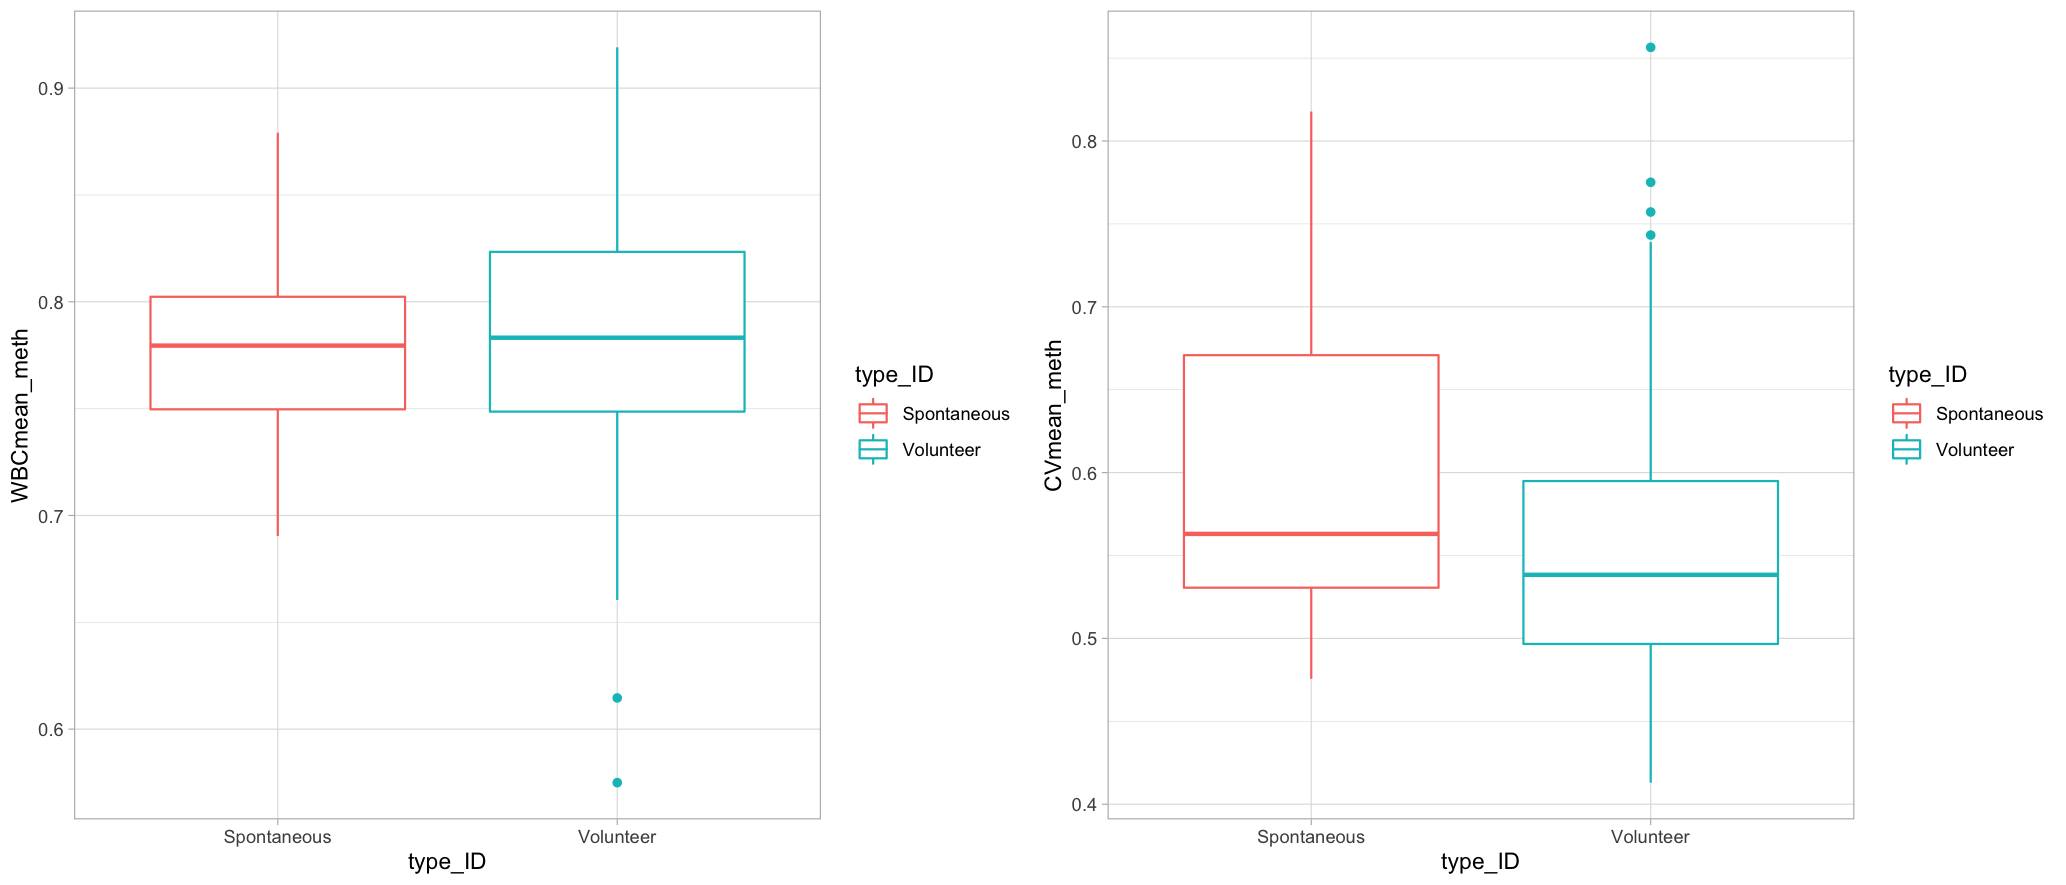
\includegraphics[width=16 cm]{Definitions/Global_methylation_pannello.png}
    \caption{Global methylation of LINE-1 in WBC on the left and CV on the right}
    \label{fig:Global methylation}
\end{figure}
%DA SISTEMARE GRAFICO


\begin{table}[H]
\caption{Evaluation of LINE-1 methylation in subsets based on the clinical data.}
\centering
\resizebox{\textwidth}{!}{%
\begin{tabular}{ccccccc}
\hline
\textit{\textbf{\begin{tabular}[c]{@{}c@{}} LINE-1 \\ methylation\end{tabular}}} &
  \multicolumn{3}{c}{\textit{\textbf{Analysis level of methylation in WBC}}} &
  \multicolumn{3}{c}{\textit{\textbf{Analysis level of methylation in CV}}} \\ \hline
\textit{\textbf{}} &
  \textit{\textbf{Mean $\pm$ SD}} &
  \textit{\textbf{Mean $\pm$ SD}} &
  \textit{\textbf{p-value}} &
  \textit{\textbf{Mean $\pm$ SD}} &
  \textit{\textbf{Mean $\pm$ SD}} &
  \textit{\textbf{p-value}} \\ \hline
\textit{\textbf{Mother's age 35 years}} &
  \textit{\textbf{\textgreater{}=35}} &
  \textit{\textbf{\textless{}35}} &
  \textit{} &
  \textbf{\textgreater{}=35} &
  \textbf{\textless{}35} &
  \textit{} \\ \hline
RPL                        & 77 \% \pm  0.40\%       & 78\% \pm 0.40\%     & \textit{p= 0.46} & 61\%  \pm 0.94\%      & 60\%   \pm  1.05\%     & \textit{p=0.53} \\ \hline
VTP                       & 76\%  \pm 0.53 \%          & 78\%   \pm  0.64 \%         & \textit{p=0.20} & 54\% \pm  0.78 \%      & 55\%  \pm  0.86 \%      & \textit{p=0.87} \\ \hline
\textit{\textbf{Mother's BMI}} &
  \textit{\textbf{Normal weight}} &
  \textit{\textbf{Overweight}} &
  \textit{\textbf{}} &
  \textit{\textbf{Normal weight}} &
  \textit{\textbf{Overweight}} &
  \textit{\textbf{}} \\ \hline
RPL                        & 78\% \pm 0.37\%  & 76\% \pm 0.48\%           & \textit{p=0.080} & 59\% \pm 1.0 \%        & 62\% \pm   1.0 \%      & \textit{p=0.40} \\ \hline
VTP                       & 78\% \pm  0.54 \%       & 76\%  \pm 0.70 \%       & \textit{p=0.20} & 54\% \pm 0.78 \%         & 55\% \pm   0.76 \%       & \textit{p=0.51} \\ \hline
\textit{\textbf{Smoking exposure}} &
  \textit{\textbf{"Yes"}} &
  \textit{\textbf{"No"}} &
  \textit{\textbf{}} &
  \textit{\textbf{"Yes"}} &
  \textit{\textbf{"No"}} &
   \\ \hline
RPL                        & 78\%\pm 0.38 \%     & 77\%\pm 0.39\%    & \textit{p=0.70} & 61\% \pm  1.0\%          & 59\% \pm   0.95\%        & \textit{p=0.59} \\ \hline
VTP                       & 79\% \pm  0.46\%       & 75 \% \pm 0.69\%       & \textit{{p=0.060}} & 54\% \pm    0.89\%       & 54\%  \pm    0.71\%     & \textit{p=0.79} \\ \hline
\textit{\textbf{Embryo's age}} &
  \textit{\textbf{\textgreater{}70}} &
  \textit{\textbf{\textless{}=70}} &
  \textit{\textbf{}} &
  \textit{\textbf{\textgreater{}70}} &
  \textit{\textbf{\textless{}=70}} &
   \\ \hline
RPL                        & 78\%  \pm 0.42\%        & 77\% \pm 0.41\%         & \textit{p=0.36} & 58\% \pm  0.9\%        & 62\% \pm 1.0\%         & \textit{p=0.06} \\ \hline
VTP                       & 79\% \pm 0.5\%         & 76\% \pm  0.6\%         & \textit{p= 0.06} & 53\% \pm  0.9\%        & 56\% \pm  0.8\%         & \textit{p=0.10} \\ \hline
\textit{\textbf{Folic acid}} &
  \textit{\textbf{"Yes"}} &
  \textit{\textbf{"No"}} &
  \textit{} &
  \textbf{"Yes"} &
  \textbf{"No"} &
  \textit{} \\ \hline
RPL                        & 77\% \pm 0.45\%         & 77\% \pm 0.38 \%          & \textit{p= 0.97} &    57\% \pm 0.81\%     &   62\% \pm 1.0\%       & \textit{\textbf{p= 0.030}} \\ \hline
VTP                       & NA           & NA           & \textit{NA} &  NA         & 78\% \pm 0.56 \%         & \textit{NA} \\ \hline
\textit{\textbf{Embryo's sex}} &
  \textit{\textbf{"Female"}} &
  \textit{\textbf{"Male"}} &
  \textit{\textbf{}} &
  \textit{\textbf{"Female"}} &
  \textit{\textbf{"Male"}} &
  \textit{} \\ \hline
RPL                        & 78\% \pm 0.41 \%         & 77\%\pm 0.45 \%          & \textit{p=0.76} & 61\%   \pm  1.0\%     & 60\% \pm 0.80\%         & \textit{p=0.86} \\ \hline
VTP                       & 78\% \pm 0.54\%
& 77 \% \pm 0.67 \%        & \textit{p=0.40} & 56\%  \pm 1.0 \%      & 54\% \pm   0.68 \%       & \textit{p=0.67} \\ \hline
\end{tabular}}
\label{tab:LINE-1 methylation on clinical data}
\end{table}

%Text

%Text

%\begin{table}[H]
%\caption{This is a table caption. Tables should be placed in the main text near to the first time they are cited.}
%\centering
%\tablesize{} %% You can specify the fontsize here, e.g., \tablesize{\footnotesize}. If commented out %\small will be used.
%\begin{tabular}{ccc}
%\toprule
%\textbf{Title 1}	& \textbf{Title 2}	& \textbf{Title 3}\\
%\midrule
%entry 1		& data			& data\\
%entry 2		& data			& data\\
%\bottomrule
%\end{tabular}
%\end{table}

%Text

%Text

%\begin{listing}[H]
%\caption{Title of the listing}
%\rule{\textwidth}{1pt}
%\raggedright Text of the listing. In font size footnotesize, small, or normalsize. Preferred format: left aligned and single spaced. Preferred border format: top border line and bottom border line.
%\rule{\textwidth}{1pt}
%\end{listing}


%\subsection{Formatting of Mathematical Components}

%This is an example of an equation:

%\begin{equation}
%a + b = c
%\end{equation}
%% If the documentclass option "submit" is chosen, please insert a blank line before and after any math environment (equation and eqnarray environments). This ensures correct linenumbering. The blank line should be removed when the documentclass option is changed to "accept" because the text following an equation should not be a new paragraph. 

%Please punctuate equations as regular text. Theorem-type environments (including propositions, lemmas, corollaries etc.) can be formatted as follows:
%% Example of a theorem:
%\begin{Theorem}
%Example text of a theorem.
%\end{Theorem}

%The text continues here. Proofs must be formatted as follows:

%% Example of a proof:
%\begin{proof}[Proof of Theorem 1]
%Text of the proof. Note that the phrase `of Theorem 1' is optional if it is clear which theorem is being referred to.
%\end{proof}
%The text continues here.

%%%%%%%%%%%%%%%%%%%%%%%%%%%%%%%%%%%%%%%%%%
\section{Discussion}

%Authors should discuss the results and how they can be interpreted in perspective of previous studies and of the working hypotheses. The findings and their implications should be discussed in the broadest context possible. Future research directions may also be highlighted.

\noindent In this study, we want to investigate genetics and epigenetics of recurrent pregnancy loss through the analysis of genetic markers from genes which have been demonstrated to play an important role in this pathology. This study is quite unique, as it is one of few which had investigated gDNA methylation in tissue from CV of recurrent spontaneous abortion cases using samples from VTP as reference controls.


\subsection{Genetic of miscarriage}

\noindent This preliminary study suggests that risk of RPL is influenced by maternal's genotype. In particular, the recessive allele of the SNP \textit{MTHFR} c.677C>T seems to have an effect on the risk of RPL, with triplicate risk in T/T homozygous women and half risk in heterozygous. We hypothesize that this evidence could be related to reduced synthesis of 5- methyl-Tetrahydrofolate in T/T homozygotes \cite{jacques1996relation}, which could eventually dysregulates the methylation of genomic DNA, ultimately leading to epigenetic modifications, which could affect the survival of embryos. In fact, in this epigenetic study related to comparison between \textit{MTHFR}c.677C>T and global level of LINE-1, we see a trend of significance difference in methylation between wild type genotype and heterozygous and recessive homozygous genotype. This evidence needs further investigations in a larger case-control cohort, especially because the allele T might be causes increase of risk RPL in population, especially in Italian population. In fact, this could be related to increased prevalence of T/T genotype in Italian's one, as shown by study of Wilcken et al., 2003 \cite{wilcken2003geographical}, where he saw in 12-15\% of cases of T/T genotype in southern Europe (Spain and northern Italy), peaking in southern Italy (20-26\% in Campania and Sicily).\\

\noindent In this study, an important role in reduce the risk of RPL in the embryo, seems to play the \textit{NKG2D} gene (rs2617170). In the analysis of ORs based on alleles, the recessive allele A gives protection (p=0.025). The same effect can be seen on recessive genotype where the effect of reduction of RPL be increase ( p=0.0067). In a study from \textit{Hizem et al.,2014} \cite{hizem2014polymorphisms}, the recessive genotype in mothers is correlated with higher cytotoxic activity. Here for the first time we observe the effects on embryos is opposite, i.e. protection from RPL. In a normal pregnancy, the role of \textit{NKG2D} is to stimulate decidual NK cells to produce a type of cytokines that induce angiogenesis, such as vascular endothelium that contributes to the uterine vascular re-modeling. Indeed, the fetus itself is never in direct contact with uterine tissues and maternal blood. The role to invade the decidua and form the placenta is of fetal trophoblast and the cytokines, secreted by maternal and fetal cells at the site of implantation, contribute to maintain the communication between trophoblast and decidual cells. This help to maintain in balance the fetal interface and the maternal immune system in normal pregnancy. Syncytiotrophoblast cells produce and secrete NKG2D ligands via exosomes. The NKG2D ligand-loaded exosomes in normal pregnancy serum is able to interact with NKG2D and downregulate the receptor expression on peripheral blood mononuclear cells (PBMC), with the following inhibition of the NKG2D-dependent cytotoxic response. The presence of this recessive genotype in embryos, probably can contribute to maintain this secretion by syncytiotrophoblast's cells \cite{mei2012defects}.\\

\subsection{Epigenetic in miscarriage}

\noindent The term epigenetic  refers  to  the  study  of  alterations in  gene  function  that  are mitotically and/or meiotically heritable and that do not entail a change in the DNA sequence. Epigenetic mechanisms are essential for development and differentiation, but can be disrupted by exogenous factors \cite{godderis2015global}. Scientific evidence increasingly suggests that exposures during the intrauterine period can increase the danger of developing disease in later life \cite{breton2009prenatal}. In this study, we examined the DNA methylation in the samples of gDNA from both in WBC and CV. We want to understand if the life style of the mothers (e.g. smoke, alcool, folic acid intake) can influence the environment of pregnancy. In particular, we want to understand if a bad life style can cause RPL. We evaluated the role of epigenetic in RPL through the analysis of LINE-1 methylation. Because of their high genome dissemination, LINE-1 methylation is a good surrogate marker of global DNA methylation level. This study is quite unique, as it is one of few which investigated gDNA methylation in tissue from CV of recurrent pregnancy loss cases. The preliminary results show no significant LINE-1 methylation difference between gDNA from RPL and VTP in mother’s white blood cells (WBC). However, a significant increase of 5\% higher methylation level (p-value 0.0010) can be seen in RPL cases compared to VTP cases when considering gDNA from chorionic villi. This results, although preliminary, provide for the first time evidence of an increased level of LINE-1 methylation in RPL cases, suggesting that altered epigenetics of the embryo could play a role in determining the recurrent pregnancy loss. This difference seems not to be influenced by mother's age, smoking exposure and BMI or embryo’s sex and age. Among VTP cases the stratification for FA supplementation exposure was not possible, due to the lack of positive cases (only one VTP case was supplemented with FA). Folate is an important precursor of one-carbon units required for DNA methylation. Thus, folate metabolism has been suggested to influence epigenetic alterations in cancer. High folic acid might contribute to the maintenance of global methylation through an equal supply of one-carbon units for the methylation machinery, thereby stabilizing the genome \cite{jin2009different}. Here an effect was observed when considering the exposure to periconceptional supplementation with folic acid (FA) (400 μg/day). As shown in Table \ref{tab:LINE-1 methylation on clinical data}, the LINE-1 DNA methylation among RPL cases in CV is significantly higher in cases not supplemented with FA (p-value = 0.030). Among VTP cases the stratification for FA supplementation exposure was not possible, due to the lack of positive cases. The result of epigenetic analysis is indicating a possible role of folate bioavailability in causing RPL, and suggesting that intervention with folate supplementation could be beneficial in preventing this pathology. In addition, to support this thesis, from stratification on different SNP, in WBC, the \textit{MTHFR} rs1801133 shows a trend of difference in mean of methylation among RPL cases, where the comparison between wild type C/C and the heterozygous and recessive genotype T/T shows a decrease of methylation in recessive genotype of 6\% (p=0.17, p=0.11). The same patterns of demethylation is seen in VTP and it became significant (p=0.01), with a decrease of methylation of 9\% in recessive genotype in VTP. This can be related to minor efficiency of enzyme activity in T/T genotype, so the lower level of methylation increase activity of the gene. 



%%%%%%%%%%%%%%%%%%%%%%%%%%%%%%%%%%%%%%%%%%
\section{Materials and Methods}

%Materials and Methods should be described with sufficient details to allow others to replicate and build on published results. Please note that publication of your manuscript implicates that you must make all materials, data, computer code, and protocols associated with the publication available to readers. Please disclose at the submission stage any restrictions on the availability of materials or information. New methods and protocols should be described in detail while well-established methods can be briefly described and appropriately cited.

%Research manuscripts reporting large datasets that are deposited in a publicly available database should specify where the data have been deposited and provide the relevant accession numbers. If the accession numbers have not yet been obtained at the time of submission, please state that they will be provided during review. They must be provided prior to publication.

%Interventionary studies involving animals or humans, and other studies require ethical approval must list the authority that provided approval and the corresponding ethical approval code. 

\subsection{Data and samples collection}

\noindent In this study were analyzed data from 156 women that underwent Voluntary Termination of Pregnancy (VTP) and 91 recurrent pregnancy loss \textbf{(RPL)}, 40 first pregnancy loss \textbf{(FPL)} in a total of 131 women experiencing Pregnancy Loss (PL). The samples were provided by the Unit of Obstetrics and Gynecology at The Sant’Anna University Hospital of Ferrara, Italy, from 2016 to 2020. The inclusion criteria were: patient’s age in the range 18–42 years, gestational age within the first 12 weeks and the cohort of VTP pregnancy was composed of females that have a volutary miscarriage until 90 days according to the Italian law, named \textit{Bill 194, Article 4}. The exclusion criteria were: patients positive for infectious agents/diseases, such as HIV, hepatitis B virus, hepatitis C virus, syphilis and the presence of congenital or acquired immune deficiency syndrome/diseases, or immunosuppressive therapies, all during the year before the sample collection. And causes of recurrent pregnancy loss as genetics, severe uterine or hormonal dysregulation, and use of teratogenic drugs. The samples were composed by the products of the conception and the relative peripheral blood of mothers. The project \textbf{G.R Reg. E/R (PRUA1GR-2013 00000220)} \textit{“Silent Intrauterine infections and early pregnancy loss”} was approved by Local Ethical Committee \textbf{(CE/FE 170475)} and was carried out in compliance with the Helsinki Declaration. All participants provided written informed consents before recruitment. Data set consists of medical data from interviews on 283 cases. In the questionnaire, there is information about mother’s age, Body Mass Index (BMI), gestational age, menarche, geographical origin, educational level, lifestyle factors (smoking, alcohol consumption, drug consumption), chronic disease, folic acid intake, obstetric and gynecologic history of mother and sister of the patient. All the data were anonymized right after data and sample collection. 

\subsection{Genomic DNA extraction, quantification and storage}
\noindent The material of conception with relative media arrives in the laboratory in sterilized Falcon tubes of 15 ml. The selection of chorionic villi from the maternal material must be done under a laminar flow hood to preserve the sterility of the sample. The most challenging step of the protocol consists of distinguishing and separating exclusively the villi from the rest of the maternal material like placenta, and decidua. The dissection takes place under the hood using a stereomicroscope (e.g. Leica Microsystems Srl, All Microscopy and Histology, Milan, I-20142 Italy).  The operator should recognize chorionic villi at the stereomicroscope and separate them from the decidua using scalpels. The villi can be stored at -20 \si{\degree}C in vials, for a few months or at 4\si{\degree}C in RPMI media for not more than a week before proceeding to DNA extraction. The peripheral blood from mothers was collected in tubes with EDTA at the same time of collection of the miscarriage material. Genomic DNA (gDNA) was extracted from chorionic villi dissected from abortion tissue specimens using QIAamp DNA Blood Mini Kit (Qiagen) in according to manufacturer protocols \textit{(QIAamp DNA Mini and Blood Mini Handbook 05/2016. Instruction Manual)}. The gDNA obtained from white blood cell (WBC) of peripheral blood samples from mothers was instead extracted using the Nucleon BACC1 (GE Healthcare UK), according to manufacturer protocols (\textit{RPN8501-PL Rev C 04/2008}). All genomic DNA was quantified using Qubit® dsDNA BR Assay Kit (Life technologies Oregon, USA). After each gDNA was inserted in Matrix 2D-Barcoded (Thermo Fisher Scientific) and they made possible set up a DNA-Biobank located in -80\si{\degree}C freezer equipped with Access Key and constant monitoring of use and function conditions. %Working conditions took place using genomic DNA at concentrations of 10 ng/$\mu$L or 1ng/$\mu$L, depending on methodology, in order to normalize results.

\subsection{Genotyping}

\noindent The genomic DNA obtained from WBC and abortion tissue specimens were used for the genotyping of a panel of candidate gene variants with 5’- nucleus Real-Time PCR assay using allele-specific TaqMan probes. PCR conditions for all reaction were as follows: 50\si{\degree}C for 2 min, 95\si{\degree}C for 10 min and (95\si{\degree}C for 15 s, 60\si{\degree}C for 1 min) x 50 cycles. The instrument used for reading plate was Applied BioSystems ABI PRISM 7300 (Applied BioSystems, Foster City, CA). The gene HLA-G 14 bp was analyzed by a polymerase chain reaction (PCR) sequence-specific primer method (PCR-PAGE) \cite{castelli2014insights}. The amplification was performed by PCR with a GeneAmp PCR System 2700 thermal cycler (Applied Biosystems, Foster City, CA) in a 25 $\mu$L reaction mixture containing 100ng of genomic DNA, 10XPCR buffer, 50mM MgCl2, 10mM dNTPs, 20pmol of each primer and 1U of Taq polymerase (Invitrogen Co., Carlsbad, Ca). The PCR conditions comprised initial denaturation at 94\si{\degree}C for 2 min, followed by 10 cycles of denaturation at 94\si{\degree}C for 15 s, annealing at 64\si{\degree}C for 30 s and extension at 72\si{\degree}C for 30 s, then 25 cycles of denaturation at 94\si{\degree}C for 15 s, annealing at 63\si{\degree}C for 30 s and extension at 72\si{\degree}C for 30 s, and final extension at 72\si{\degree}C for 5 min. The purified PCR products size were analyzed using an 8\% polyacrylamide gel. The product size was 224 bp for Ins/Ins (I/I) and 210 bp for Del/Del (D/D) and both 224 bp and 210 bp for Del/Ins (D/I) genotypes. The PCR products were visualized using silver staining. 

\subsection{Pyrosequencing}

\noindent This protocol is in accord to study of Khan MFJ. et al., 2017 \cite{khan2018evaluating}. The genomic DNA samples were next bisulfite-converted using EZ DNA Methylation-Lightning Kit (Zymo Research, Irvine, CA, USA), according to manufacturer's instructions (Instruction manual CAT. No. D5030T, ver 1.0.4). After that, the CpG islands of LINE-1 sequences were amplified by PCR. The PCR reactions were performed with a total volume of 25 $\mu$L containing: 10X PCR Buffer, 50mM MgCl2, 2.5 mM dNTPs, 10 pM Reverse Primer LINE-1, 10 pM Forward Primer LINE-1, 5U Taq-Polymerase and 2.5 $\mu$L of Bisulfite DNA. The cycling profile was composed of 27 cycles of 94 \si{\celsius} for 15 sec, 60\si{\celsius} for 30 sec and 72\si{\celsius} for 30 sec, followed by 72\si{\celsius} for 2 min. The amplicon of 147 bp was analyzed on 8\% polyacrylamide gel using silver staining. The products of PCR were sequenced by pyrosequencing using the PyroMark Q96 system (Qiagen), according to manufacturer’s instructions (PyroMark Q96 ID User Manual 01/2016). The average of LINE-1 methylation level was calculated as of the mean of the proportions of C (\%) at the 4 CpG sites analyzed, which were located at positions +306, +318, +321 and +328 (positions of the corresponding Guanine in the forward DNA strand, in relation to the first nucleotide base of the consensus promoter sequence in Genebank sequence no. X58075, position 305-331), represented in the red rectangles.

\subsection{Statistical analysis}

\noindent The analyses done follows the guidelines for statistical analysis for case-control study of \textit{Clarke GM. et al.,2011} \cite{clarke2011basic}. All the statistical analyses were performed using the R studio software (R studio version 3.6.2). The Hardy-Weindberg equilbrium (HWE) was tested with "Hardy- Weinberg" package in R studio \cite{graffelman2015exploring}. Odds ratios (ORs) and 95\% confidence intervals (95\% CIs) were estimated on nine SNPs with MAF > 5-10\%.A z-test was applied, and a two-tailed p-value less than 0.05 was considered statistically significant. ORs were calculated for genotypes and alleles, assuming a co-dominant genetic model. Methylation scores of the LINE-1 sequence was calculated as the average over all 4 CpG islands in a sample. The distribution of LINE-1 methylation levels were checked for normality using the Shapiro-Wilk test. For WBC samples that not departed from normality, as parametric test, an unpaired t-student test was used to test the significativity. For CV samples, we used a non parametric test called "\textit{Mann-Whitney}". A t-student test was used for WBC and Mann-Whitney for CV, to evaluate the difference of average of methylation with a stratification on several parameters included in the clinical database, the same for OR. All p-values were two sided, with a threshold for declaring statistical significance of p < 0.05. \\



%%%%%%%%%%%%%%%%%%%%%%%%%%%%%%%%%%%%%%%%%%
\section{Conclusions}

%This section is not mandatory, but can be added to the manuscript if the discussion is unusually long or complex.

\noindent This preliminary study indicate that risk of RPL is influenced by maternal \textit{MTHFR} c.677C>T genotypes. In conclusion this study suggests a possible causal role due to unbalanced folate metabolism, and lays the groundwork for innovative measures aimed at preventing recurrence of spontaneous abortion. In the embryos, available for the first time, we see a protective effect at the \textit{NKG2D} gene. This study give the important information that it is important to study, not only the maternal genome, but also the fetal genome, an aspect that has been neglected until now. This results, although preliminary, provide for the first time evidence of an increased level of LINE-1 methylation in RPL cases, suggesting that altered epigenetics of the embryo could play a role in determining the recurrent pregnancy loss. Moreover, we provide first evidence of an influence of mother’s periconceptional exposure to folic acid supplementation on the global genomic methylation level of embryo’s chorionic villi, indicating a possible role of folate bioavailability in causing RPL, and suggesting that intervention with folate supplementation could be beneficial in preventing this pathology. As future direction, this study shows the importance to focus on the trios (mother, father and fetus) during pregnancy in order to prevent miscarriage. Acting on mother life style where this are not suitable for good result of pregnancy. This results lay the foundations for identifying an effective protocol for the treatment of women with recurrent spontaneous abortion without apparent cause, that currently is absent.

%%%%%%%%%%%%%%%%%%%%%%%%%%%%%%%%%%%%%%%%%%
%\section{Patents}
%This section is not mandatory, but may be added if there are patents resulting from the work reported in this manuscript.

%%%%%%%%%%%%%%%%%%%%%%%%%%%%%%%%%%%%%%%%%%
\vspace{6pt} 

%%%%%%%%%%%%%%%%%%%%%%%%%%%%%%%%%%%%%%%%%%
%% optional
%\supplementary{The following are available online at \linksupplementary{s1}, Figure S1: title, Table S1: title, Video S1: title.}

% Only for the journal Methods and Protocols:
% If you wish to submit a video article, please do so with any other supplementary material.
% \supplementary{The following are available at \linksupplementary{s1}, Figure S1: title, Table S1: title, Video S1: title. A supporting video article is available at doi: link.}

%%%%%%%%%%%%%%%%%%%%%%%%%%%%%%%%%%%%%%%%%%
\authorcontributions{For research articles with several authors, a short paragraph specifying their individual contributions must be provided. The following statements should be used ``conceptualization, X.X. and Y.Y.; methodology, X.X.; software, X.X.; validation, X.X., Y.Y. and Z.Z.; formal analysis, X.X.; investigation, X.X.; resources, X.X.; data curation, X.X.; writing--original draft preparation, X.X.; writing--review and editing, X.X.; visualization, X.X.; supervision, X.X.; project administration, X.X.; funding acquisition, Y.Y.'', please turn to the  \href{http://img.mdpi.org/data/contributor-role-instruction.pdf}{CRediT taxonomy} for the term explanation. Authorship must be limited to those who have contributed substantially to the work reported.}

%%%%%%%%%%%%%%%%%%%%%%%%%%%%%%%%%%%%%%%%%%
\funding{Please add: ``This research received no external funding'' or ``This research was funded by NAME OF FUNDER grant number XXX.'' and  and ``The APC was funded by XXX''. Check carefully that the details given are accurate and use the standard spelling of funding agency names at \url{https://search.crossref.org/funding}, any errors may affect your future funding.}

%%%%%%%%%%%%%%%%%%%%%%%%%%%%%%%%%%%%%%%%%%
\acknowledgments{In this section you can acknowledge any support given which is not covered by the author contribution or funding sections. This may include administrative and technical support, or donations in kind (e.g., materials used for experiments).}

%%%%%%%%%%%%%%%%%%%%%%%%%%%%%%%%%%%%%%%%%%
\conflictsofinterest{The authors declare no conflict of interest.} 

%Declare conflicts of interest or state ``The authors declare no conflict of interest.'' Authors must identify and declare any personal circumstances or interest that may be perceived as inappropriately influencing the representation or interpretation of reported research results. Any role of the funders in the design of the study; in the collection, analyses or interpretation of data; in the writing of the manuscript, or in the decision to publish the results must be declared in this section. If there is no role, please state ``The funders had no role in the design of the study; in the collection, analyses, or interpretation of data; in the writing of the manuscript, or in the decision to publish the results''.

%%%%%%%%%%%%%%%%%%%%%%%%%%%%%%%%%%%%%%%%%%
%% optional
\abbreviations{The following abbreviations are used in this manuscript:\\

\noindent 
\begin{tabular}{@{}ll}
MDPI & Multidisciplinary Digital Publishing Institute\\
DOAJ & Directory of open access journals\\
TLA & Three letter acronym\\
LD & linear dichroism
\end{tabular}}

%%%%%%%%%%%%%%%%%%%%%%%%%%%%%%%%%%%%%%%%%%
%% optional
\appendixtitles{no} %Leave argument "no" if all appendix headings stay EMPTY (then no dot is printed after "Appendix A"). If the appendix sections contain a heading then change the argument to "yes".
\appendix
\section{}
\unskip
\subsection{}
The appendix is an optional section that can contain details and data supplemental to the main text. For example, explanations of experimental details that would disrupt the flow of the main text, but nonetheless remain crucial to understanding and reproducing the research shown; figures of replicates for experiments of which representative data is shown in the main text can be added here if brief, or as Supplementary data. Mathematical proofs of results not central to the paper can be added as an appendix.

\section{}
All appendix sections must be cited in the main text. In the appendixes, Figures, Tables, etc. should be labeled starting with `A', e.g., Figure A1, Figure A2, etc. 

%%%%%%%%%%%%%%%%%%%%%%%%%%%%%%%%%%%%%%%%%%
% Citations and References in Supplementary files are permitted provided that they also appear in the reference list here. 

%=====================================
% References, variant A: internal bibliography
%=====================================
\reftitle{References}
%\begin{thebibliography}{999}
% Reference 1
%\bibitem[Author1(year)]{ref-journal}
Author1, T. The title of the cited article. {\em Journal Abbreviation} {\bf 2008}, {\em 10}, 142--149.
% Reference 2
%\bibitem[Author2(year)]{ref-book}
Author2, L. The title of the cited contribution. In {\em The Book Title}; Editor1, F., Editor2, A., Eds.; Publishing House: City, Country, 2007; pp. 32--58.
%\end{thebibliography}

% The following MDPI journals use author-date citation: Arts, Econometrics, Economies, Genealogy, Humanities, IJFS, JRFM, Laws, Religions, Risks, Social Sciences. For those journals, please follow the formatting guidelines on http://www.mdpi.com/authors/references
% To cite two works by the same author: \citeauthor{ref-journal-1a} (\citeyear{ref-journal-1a}, \citeyear{ref-journal-1b}). This produces: Whittaker (1967, 1975)
% To cite two works by the same author with specific pages: \citeauthor{ref-journal-3a} (\citeyear{ref-journal-3a}, p. 328; \citeyear{ref-journal-3b}, p.475). This produces: Wong (1999, p. 328; 2000, p. 475)

%=====================================
% References, variant B: external bibliography
%=====================================
\externalbibliography{yes}
\bibliography{name.bib}

%%%%%%%%%%%%%%%%%%%%%%%%%%%%%%%%%%%%%%%%%%
%% optional
\sampleavailability{Samples of the compounds ...... are available from the authors.}

%% for journal Sci
%\reviewreports{\\
%Reviewer 1 comments and authors’ response\\
%Reviewer 2 comments and authors’ response\\
%Reviewer 3 comments and authors’ response
%}

%%%%%%%%%%%%%%%%%%%%%%%%%%%%%%%%%%%%%%%%%%
\end{document}

